\documentclass[12pt]{article} % use larger type; default would be 10pt

\usepackage{pgfplots}
\usetikzlibrary{calc}
\usetikzlibrary{arrows}
\usetikzlibrary{patterns}
\usetikzlibrary{calc,intersections,through,backgrounds}
\usetikzlibrary{decorations.pathreplacing}
        \newcommand\degree[0]{^{\circ}}
        \newcommand\abs[1]{\left|#1\right|}

\title{Play with TikZ}
\author{Just Us}
%\date{} % Activate to display a given date or no date (if empty),
         % otherwise the current date is printed 

\begin{document}
\maketitle

\section{chapter 10 review}






hp10-rev-1ans polar plot

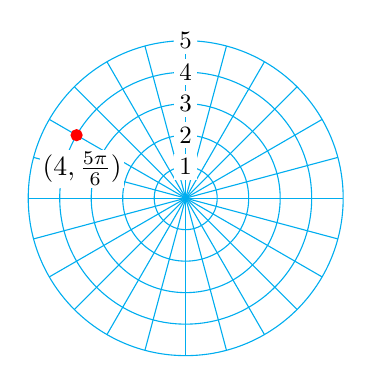
\begin{tikzpicture} [scale=.4]
\coordinate(O) at (0,0);
\foreach \angle [count=\xi] in {0, 15, ..., 345}{
  \draw[cyan] (\angle:0) -- (\angle:5);
}
\foreach \r in {1,2,3,4,5} {
\draw[cyan] (O) circle (\r);
\node[fill=white, inner sep = 2, text=black, scale=.9] at (90:\r) {$\r$};
}
\filldraw[red] (150:4) circle (5pt) node[below, xshift=2, yshift=-5, text=black, fill=white, inner sep=1]{$(4,\frac{5\pi}{6})$};
\end{tikzpicture}
\newline


hp10-rev-3ans polar plot

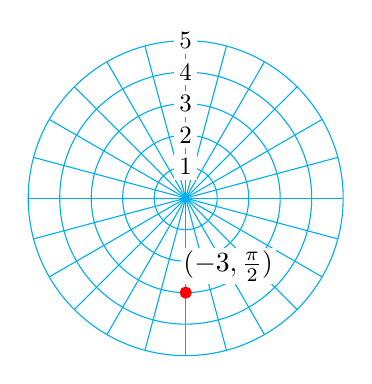
\begin{tikzpicture} [scale=.4]
\coordinate(O) at (0,0);
\foreach \angle [count=\xi] in {0, 15, ..., 345}{
  \draw[cyan] (\angle:0) -- (\angle:5);
}
\foreach \r in {1,2,3,4,5} {
\draw[cyan] (O) circle (\r);
\node[fill=white, inner sep = 2, text=black, scale=.9] at (90:\r) {$\r$};
}
\filldraw[red] (90:-3) circle (5pt) node[above right, xshift=-2, yshift=3, text=black, fill=white, inner sep=1]{$(-3,\frac{\pi}{2})$};
\end{tikzpicture}
\newline


hp10-rev-13ans polar plot


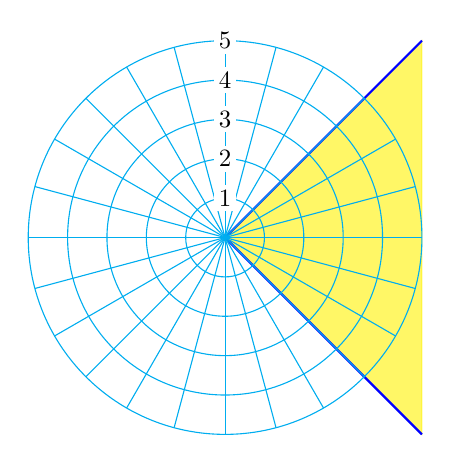
\begin{tikzpicture} [scale=.5]
\coordinate(O) at (0,0);
\filldraw [yellow, opacity = 0.6] (O)--(-45:{5*sqrt(2)}) -- (45:{5*sqrt(2)}) -- (O);
\draw[blue, thick] (-45:{5*sqrt(2)})--(O)--(45:{5*sqrt(2)});

\foreach \angle [count=\xi] in {0, 15, ..., 345}{
  \draw[cyan] (\angle:0) -- (\angle:5);
}
\foreach \r in {1,2,3,4,5} {
\draw[cyan] (O) circle (\r);
\node[fill=white, inner sep = 2, text=black, scale=.9] at (90:\r) {$\r$};
}

\end{tikzpicture}
\newline


hp10-rev-15ans

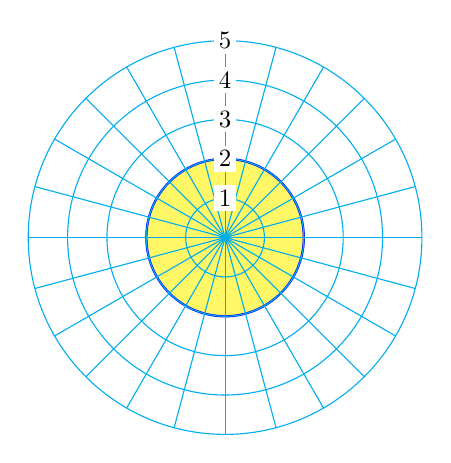
\begin{tikzpicture} [scale=.5]
\coordinate(O) at (0,0);
\draw[blue, thick, fill=yellow, fill opacity = 0.6] (O) circle (2cm);

\foreach \angle [count=\xi] in {0, 15, ..., 345}{
  \draw[cyan] (\angle:0) -- (\angle:5);
}
\foreach \r in {1,2,3,4,5} {
\draw[cyan] (O) circle (\r);
\node[fill=white, inner sep = 2, text=black, scale=.9] at (90:\r) {$\r$};
}

\end{tikzpicture}
\newline

hp10-rev-29

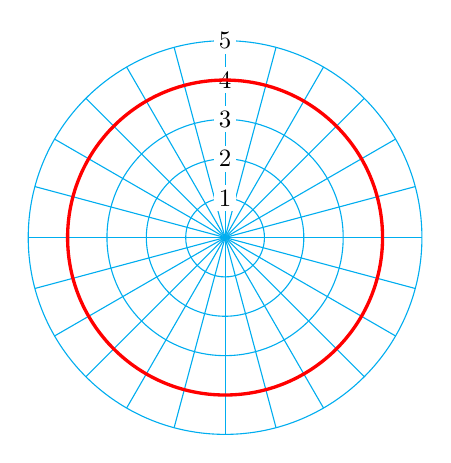
\begin{tikzpicture} [scale=.5]
\coordinate(O) at (0,0);
\foreach \angle [count=\xi] in {0, 15, ..., 345}{
  \draw[cyan] (\angle:0) -- (\angle:5);
}
\foreach \r in {1,2,3,4,5} {
\draw[cyan] (O) circle (\r);
\node[fill=white, inner sep = 2, text=black, scale=.9] at (90:\r) {$\r$};
}
\draw[red, very thick] (O) circle (4cm);

\end{tikzpicture}
\newline


hp10-rev-30

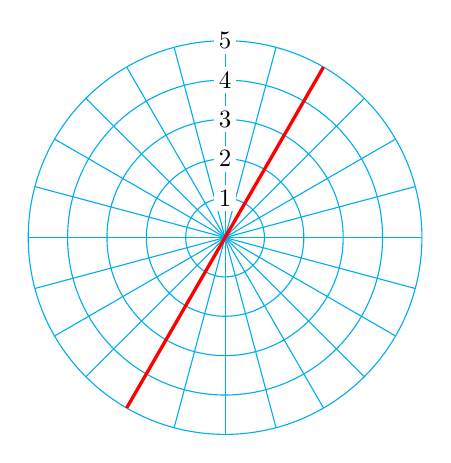
\begin{tikzpicture} [scale=.5]
\coordinate(O) at (0,0);
\foreach \angle [count=\xi] in {0, 15, ..., 345}{
  \draw[cyan] (\angle:0) -- (\angle:5);
}
\foreach \r in {1,2,3,4,5} {
\draw[cyan] (O) circle (\r);
\node[fill=white, inner sep = 2, text=black, scale=.9] at (90:\r) {$\r$};
}
\draw[red, very thick] (60:5) -- (240:5);

\end{tikzpicture}
\newline


hp10-rev-31

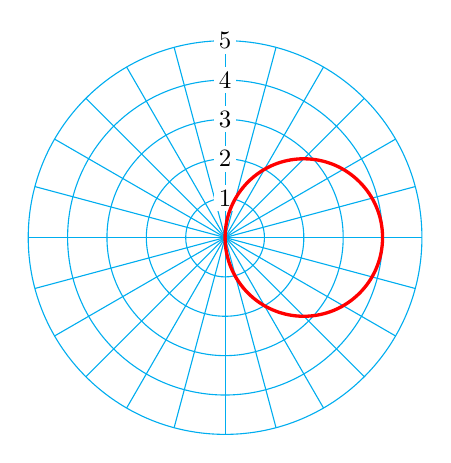
\begin{tikzpicture} [scale=.5]
\coordinate(O) at (0,0);
\foreach \angle [count=\xi] in {0, 15, ..., 345}{
  \draw[cyan] (\angle:0) -- (\angle:5);
}
\foreach \r in {1,2,3,4,5} {
\draw[cyan] (O) circle (\r);
\node[fill=white, inner sep = 2, text=black, scale=.9] at (90:\r) {$\r$};
}
\draw[red, very thick] (2,0) circle (2cm);

\end{tikzpicture}
\newline


hp10-rev-32

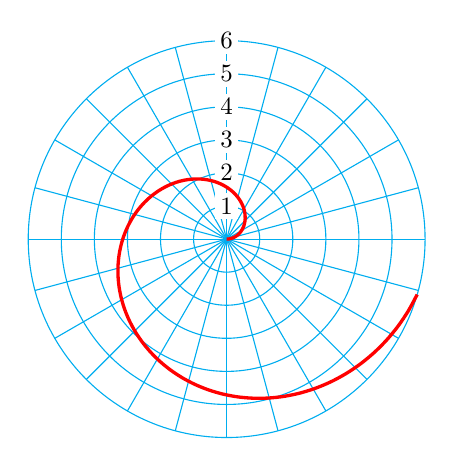
\begin{tikzpicture} [scale=.42]
\coordinate(O) at (0,0);
\foreach \angle [count=\xi] in {0, 15, ..., 345}{
  \draw[cyan] (\angle:0) -- (\angle:6);
}
\foreach \r in {1,2,3,4,5,6} {
\draw[cyan] (O) circle (\r);
\node[fill=white, inner sep = 2, text=black, scale=.9] at (90:\r) {$\r$};
}
\draw[domain=0:6,smooth, samples=65,variable=\x,red,very thick] plot ({deg(\x)}:{\x});
\end{tikzpicture}
\newline


hp10-rev-51ans rectangular grid with four complex numbers

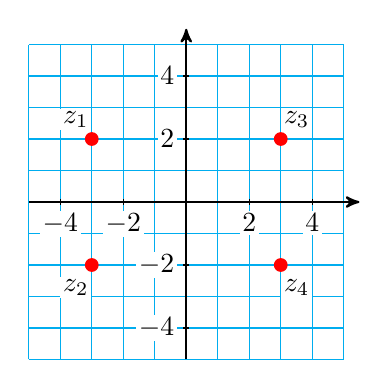
\begin{tikzpicture} [scale=.4]
\draw[cyan] (-5,-5) grid (5,5);
\draw[black, thick,->, >=stealth'] (-5,0)--(5.5,0);
\draw[black, thick,->, >=stealth'] (0,-5)--(0,5.5);
\foreach \x in {-4,-2,2,4}{
  \draw[black] (\x,0.1) --++(0,-.2) node[below, fill=white, inner sep=1, yshift=-2]{$\x$};
  \draw[black] (0.1,\x) --++(-.2,0) node[left, fill=white, inner sep=1, xshift=-2]{$\x$};
}
\draw[red, fill=red] (-3,2) circle (.2cm) node[above left, yshift=3, fill=white, inner sep=1, text=black]{$z_1$};
\draw[red, fill=red] (-3,-2) circle (.2cm) node[below left, yshift=-4, fill=white, inner sep=1, text=black]{$z_2$};
\draw[red, fill=red] (3,2) circle (.2cm) node[above right, yshift=3, fill=white, inner sep=1, text=black]{$z_3$};
\draw[red, fill=red] (3,-2) circle (.2cm) node[below right, yshift=-4, fill=white, inner sep=1, text=black]{$z_4$};
\end{tikzpicture}
\newline


hp10-rev-75ans

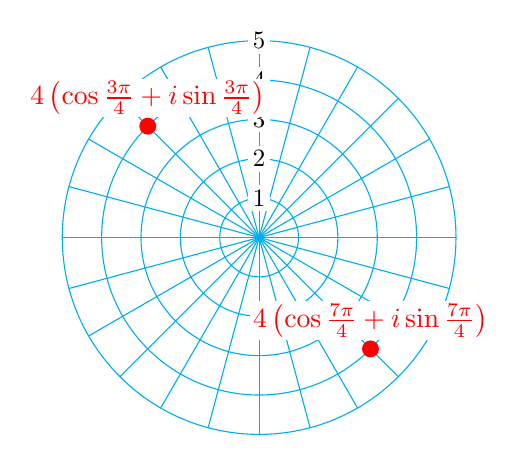
\begin{tikzpicture} [scale=.5]
\coordinate(O) at (0,0);
\foreach \angle [count=\xi] in {0, 15, ..., 345}{
  \draw[cyan] (\angle:0) -- (\angle:5);
}
\foreach \r in {1,2,3,4,5} {
\draw[cyan] (O) circle (\r);
\node[fill=white, inner sep = 2, text=black, scale=.9] at (90:\r) {$\r$};
}
\draw[red, fill=red] (135:4) circle (.2cm) node[above, yshift=3, fill=white, inner sep=1] {$4\left(\cos\frac{3\pi}{4} + i\sin\frac{3\pi}{4}\right)$};
\draw[red, fill=red] (-45:4) circle (.2cm) node[above, yshift=3, fill=white, inner sep=1] {$4\left(\cos\frac{7\pi}{4} + i\sin\frac{7\pi}{4}\right)$};

\end{tikzpicture}
\newline


hp10-rev-75ans

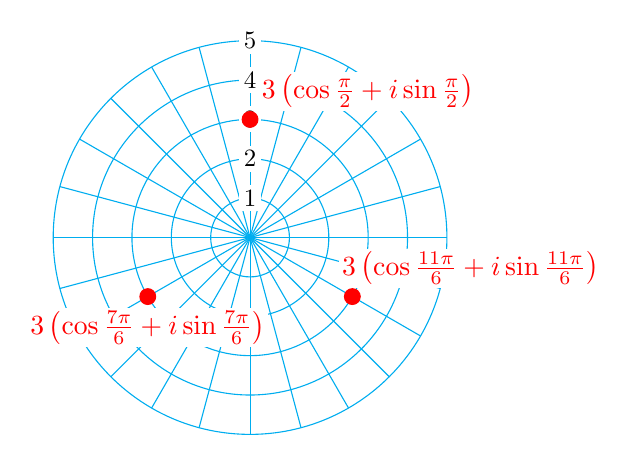
\begin{tikzpicture} [scale=.5]
\coordinate(O) at (0,0);
\foreach \angle [count=\xi] in {0, 15, ..., 345}{
  \draw[cyan] (\angle:0) -- (\angle:5);
}
\foreach \r in {1,2,3,4,5} {
\draw[cyan] (O) circle (\r);
\node[fill=white, inner sep = 2, text=black, scale=.9] at (90:\r) {$\r$};
}
\draw[red, fill=red] (90:3) circle (.2cm) node[above, xshift=1.5cm, yshift=3, fill=white, inner sep=1] {$3\left(\cos\frac{\pi}{2} + i\sin\frac{\pi}{2}\right)$};
\draw[red, fill=red] (210:3) circle (.2cm) node[below, yshift=-4, fill=white, inner sep=1] {$3\left(\cos\frac{7\pi}{6} + i\sin\frac{7\pi}{6}\right)$};
\draw[red, fill=red] (-30:3) circle (.2cm) node[above, xshift=1.5cm, yshift=3, fill=white, inner sep=1] {$3\left(\cos\frac{11\pi}{6} + i\sin\frac{11\pi}{6}\right)$};

\end{tikzpicture}
\newline






\end{document}
